\section{Implémentation}

\subsection{Architecture logicielle}
L'implémentation suit une architecture modulaire avec une séparation claire des responsabilités, organisée en trois niveaux principaux.

\begin{figure}[h]
    \centering
    \begin{tikzpicture}[
        block/.style={rectangle,draw,fill=primaryblue!20,minimum width=2.5cm,minimum height=1cm},
        subblock/.style={rectangle,draw,fill=primaryblue!10,minimum width=2cm,minimum height=0.8cm},
        arrow/.style={->,thick},
        ]
        
        % Niveau 1 : Programme principal
        \node[block] (main) at (0,2) {Programme principal (main.f90)};
        
        % Niveau 2 : Modules principaux
        \node[block] (solvers) at (-4,0) {Solveurs};
        \node[block] (parareal) at (0,0) {Parareal};
        \node[block] (domain) at (4,0) {Décomposition};
        
        % Niveau 3 : Sous-modules
        \node[subblock] (rk4) at (-6,-2) {RK4};
        \node[subblock] (ab) at (-4,-2) {AB2/AB3};
        \node[subblock] (euler) at (-2,-2) {Euler};
        \node[subblock] (mpi) at (0,-2) {MPI};
        \node[subblock] (conv) at (2,-2) {Convergence};
        \node[subblock] (deriv) at (4,-2) {Dérivées};
        
        % Connexions niveau 1-2
        \draw[arrow] (main) -- (solvers);
        \draw[arrow] (main) -- (parareal);
        \draw[arrow] (main) -- (domain);
        
        % Connexions niveau 2-3
        \draw[arrow] (solvers) -- (rk4);
        \draw[arrow] (solvers) -- (ab);
        \draw[arrow] (solvers) -- (euler);
        \draw[arrow] (parareal) -- (mpi);
        \draw[arrow] (parareal) -- (conv);
        \draw[arrow] (domain) -- (deriv);
        
        % Connexions horizontales
        \draw[arrow, dashed] (rk4) -- (mpi);
        \draw[arrow, dashed] (ab) -- (mpi);
        \draw[arrow, dashed] (euler) -- (mpi);
    \end{tikzpicture}
    \caption{Architecture détaillée du système}
    \label{fig:architecture_detailed}
\end{figure}

\begin{figure}[H]
    \centering
    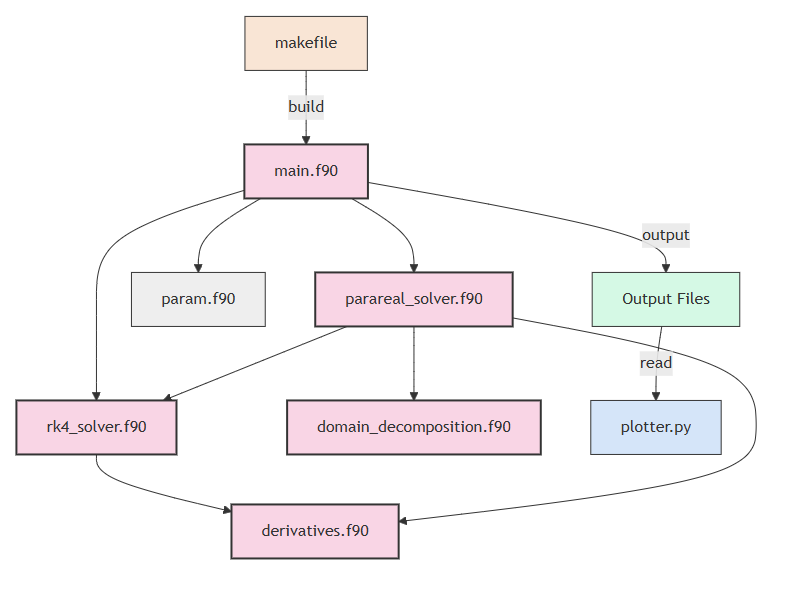
\includegraphics[width=0.8\textwidth]{code/figure.png}
    \caption{Architecture logicielle : modules et sous-modules}
    \label{fig:architecture}
\end{figure}

\subsection{Composants principaux}

\subsubsection{Programme principal (main.f90)}
Point d'entrée centralisant :
\begin{itemize}
    \item Gestion des arguments et configurations
    \item Initialisation MPI et distribution des tâches
    \item Coordination des solveurs et mesure des performances
\end{itemize}

\subsubsection{Module de solveurs}
Implémente trois niveaux de solveurs :

\begin{enumerate}
    \item \textbf{Solveur fin (RK4)} :
    \begin{itemize}
        \item Haute précision pour les calculs critiques
        \item Adaptation automatique du pas de temps
        \item Détection et gestion des instabilités
    \end{itemize}

    \item \textbf{Solveurs intermédiaires (AB2/AB3)} :
    \begin{itemize}
        \item Compromis précision/performance
        \item Stabilisation par amortissement
        \item Mélange avec l'historique pour les régimes chaotiques
    \end{itemize}

    \item \textbf{Solveur grossier (Euler)} :
    \begin{itemize}
        \item Rapidité d'exécution pour les prédictions initiales
        \item Robustesse pour les grands pas de temps
        \item Adaptation aux différents régimes de $\tau$
    \end{itemize}
\end{enumerate}

\subsection{Mécanismes de stabilité et sécurité}

\subsubsection{Adaptation aux régimes dynamiques}
Le système ajuste automatiquement ses paramètres selon la valeur de $\tau$ :

\begin{lstlisting}[language=Fortran,caption=Adaptation dynamique des paramètres]
if (tau < 1.0) then  ! Régime non-marcheur
    h_coarse = min(h_coarse, tau/20.0)
    h_fine = min(h_fine, tau/200.0)
    adapt_tol = min(tol, 1.0E-5)
else if (tau < 3.0) then  ! Marche régulière
    h_coarse = min(h_coarse, tau/10.0)
    h_fine = min(h_fine, tau/100.0)
    adapt_tol = min(tol, 5.0E-6)
else  ! Régimes chaotiques
    h_coarse = min(h_coarse, 0.1)
    h_fine = min(h_fine, 0.01)
    adapt_tol = min(tol, 1.0E-6)
end if
\end{lstlisting}

\subsubsection{Mécanismes de protection}
Implémentation de plusieurs niveaux de sécurité :

\begin{lstlisting}[language=Fortran,caption=Circuit breaker pour les instabilités]
if (any(isnan(u)) .or. any(abs(u) > MAX_VALUE)) then
    bad_value_counter = bad_value_counter + 1
    where (isnan(u)) u = 0.0
    where (abs(u) > MAX_VALUE) 
        u = sign(MAX_VALUE, u)
    end where
    
    if (bad_value_counter >= MAX_BAD_ITER) then
        status = ERROR_UNSTABLE
        return
    end if
end if
\end{lstlisting}

\subsection{Parallélisation avancée}
\subsubsection{Distribution et équilibrage}
La décomposition temporelle utilise une stratégie adaptative :

\begin{lstlisting}[language=Fortran,caption=Distribution des intervalles]
subroutine distribute_intervals(total_intervals, size, rank, 
                              start_idx, end_idx)
    integer, intent(in) :: total_intervals, size, rank
    integer, intent(out) :: start_idx, end_idx
    integer :: base_count, remainder
    
    base_count = total_intervals / size
    remainder = mod(total_intervals, size)
    
    if (rank < remainder) then
        start_idx = rank * (base_count + 1) + 1
        end_idx = start_idx + base_count
    else
        start_idx = rank * base_count + remainder + 1
        end_idx = start_idx + base_count - 1
    end if
end subroutine distribute_intervals
\end{lstlisting}

\subsection{Visualisation et analyse}
Le système inclut des capacités avancées de visualisation :

\begin{itemize}
    \item Génération de trajectoires denses adaptées au régime :
    \begin{itemize}
        \item 50 points/intervalle pour $\tau$ < 2.0
        \item 75 points/intervalle pour 2.0 $\leq$ $\tau$ < 5.0
        \item 100 points/intervalle pour $\tau$ $\geq$ 5.0
    \end{itemize}
    \item Sauvegarde structurée des résultats pour post-traitement
    \item Scripts d'analyse automatisés pour validation
\end{itemize}

\subsection{Stratégies de convergence avancées}
L'algorithme implémente plusieurs stratégies sophistiquées pour assurer et accélérer la convergence :

\subsubsection{Critère de convergence adaptatif}
Le système utilise une métrique composite pour évaluer la convergence :

\begin{lstlisting}[language=Fortran,caption=Critère de convergence hybride]
! Changement d'état relatif
rel_state_change = max_diff / (maxval(abs(U_n)) + 1.0E-10)

! Conservation de l'énergie
rel_energy_change = abs(energy_k - energy_k_prev) 
                   / (abs(energy_k_prev) + 1.0E-10)

! Métrique combinée
conv_metric = max(rel_state_change, rel_energy_change)
converged = conv_metric < adapt_tol
\end{lstlisting}

\subsubsection{Prédiction améliorée}
Pour les régimes difficiles, une stratégie d'extrapolation est utilisée :

\begin{lstlisting}[language=Fortran,caption=Extrapolation pour prédiction]
if (k > 1) then
    ! Utilisation de l'historique des corrections
    U_new = propagate_with_ab3(...) + 
            beta * (U_n - U_prev)
    
    ! Stabilisation pour les petits tau
    if (tau < 1.0) then
        U_new = 0.8 * u_coarse_new + 
                0.2 * (u_fine - u_coarse_prev + u_coarse_new)
    end if
end if
\end{lstlisting}


L'ensemble du code implémenté est disponible en accès libre sur le dépôt GitHub suivant : https://github.com/KyFaxTeam/Parareal-Lorenz. 
